\documentclass[aspectratio=1610,10pt,dvipsnames]{beamer}
\usepackage[T1]{fontenc}
\usepackage[utf8]{inputenc}
\usepackage[varg]{txfonts}
\usepackage[french]{babel}
\usepackage{multicol} % À ajouter dans le préambule

\usetheme{Ilmenau}
%%\usetheme{Copenhagen}
%%\usetheme{PaloAlto}
%%\usetheme{Antibes}
%%\usetheme{Warsaw}

\setbeamercovered{transparent}
\setbeamertemplate{footline}[frame number]
%%\usecolortheme[named=green]{structure}

\addtobeamertemplate{footline}{\insertframenumber/\inserttotalframenumber}


\title{L'instant Brain Fuck}
\date{2026}
\institute{CEA}
\author{Philippe DENIEL (philippe.deniel@cea.fr)}


\begin{document}

\frame{\titlepage}

\begin{frame}{Nombres premiers gaussiens}
Le nombre $5$ est-il entier ? On peut remarquer que 
\begin{equation*}
    5 = 4 + 1 = 2^2-i^2 = (2-i)(2+i)
\end{equation*}
5 est premier dans l'anneau $\mathbb{Z}$ mais pas dans l'anneau $\mathbb{Z}[i]$.
\\[0.5em]
Un entier premier dans $\mathbb{Z}[i]$ est un \textbf{nombre premier de Gauss}. 
\\[0.5em]
Les nombres premiers non gaussiens sont la somme de deux carrés dans $\mathbb{Z}$, on peut démontrer 
que ces nombres sont congruents à $1$ modulo $4$ (ainsi on a $5 \equiv 1 [4]$).
\end{frame}

\begin{frame}{Comment diviser par 7 facilement ?}

Il faut se rappeler que $1/7 = 0,142857142857\cdots = 0,\overline{142857}$
\\[0.3em]
La valeur décimale présente une période de 6 chiffres, or $142857$ a une propriété fascinante : c'est 
un nombre \textbf{multicyclique}.
\begin{multicols}{2}
\begin{itemize}
    \item 142857 x 1 = 142857
    \item 142857 x 2 = 285714
    \item 142857 x 3 = 428571
    \columnbreak
    \item 142857 x 4 = 571428
    \item 142857 x 5 = 714285
    \item 142857 x 6 = 857142
\end{itemize}
\end{multicols}
Les multiples de 142857 s'écrivent avec les mêmes chiffres, dans le même ordre, à une permutation circulaire
près. 
\\[0.2em]
Il suffit de se rappeler l'ordre des chiffres de 142857, soit 1, 2, 4, 5, 7, 8 pour savoir calculer toutes les
valeurs de $1/7$ à $6/7$. Ainsi $5/7 = 0,\overline{714285}$.
\\[0.2em]
À titre d'exemple, $22/7 = 21/7 + 1/7 = 3 + 1/7 = 3,\overline{142857}$, c'est une approximation de $\pi$
utilisée au temps des pharaons et connue d'Archimède. 
\\[0.2em]
Cela marche aussi pour diviser par $17$ en se rappelant la période $0,0588235294117647\dots$
\end{frame}

\begin{frame}{e à la puissance $\pi$}
À quatre décimales près, $e^\pi \approx 20 + \pi$.
\\[2cm]
\begin{equation*}
\begin{split}
    e^{\pi} &- \pi = 19,999099792\cdots \\
    e^{\pi} &- \pi = 20 - 0,00090002082834
\end{split}
\end{equation*}

\end{frame}

\begin{frame}{Puissance de $e$ et $\pi$}
On a 
\begin{equation*}
\begin{split}
    \pi^4 + \pi^5 &\approx e^6 \textrm{ à 5 décimales près} \\
    \pi^4 + \pi^5 &= e^6 - 1,76734512321 \times 10^{-5} \\
\end{split}
\end{equation*}
On a aussi
\begin{equation*}
\begin{split}
    \pi ^{\sqrt[{3}]{93}}-\mathrm {e} ^{\sqrt[{3}]{93}} &= 86{,}0000188811\dots \\
     \pi ^{\sqrt[{3}]{93}}-\mathrm {e} ^{\sqrt[{3}]{93}} &\approx 86 + 1,8 \times 10^{-5} \\
\end{split} 
\end{equation*}
\end{frame}

\begin{frame}{Un grand nombre premier de Mersenne}
En novembre 2024, le plus grand nombre premier connu était 
\\[1cm]
\begin{equation*}
    2^{136279841} - 1    
\end{equation*}
\\[1cm]
C'est un nombre de Mersenne, de la forme $M_n = 2^n - 1$.

Un nombre \textbf{parfait} est un nombre qui est égal à la somme de ses diviseurs stricts. 
\\[0.5em]
Dès le IVe siècle av. J.-C., Euclide démontrait que si $M_p$ est un nombre premier, alors 
$M_{p}(M_{p} + 1)/2 = 2^{p-1}(2^{p}-1)$ est un nombre parfait. 
\\[0.5em]
Deux millénaires plus tard, au XVIIIe siècle, Euler prouvait que tous les nombres parfaits pairs sont de 
cette forme. Par ailleurs, aucun nombre parfait impair n'est connu.
\end{frame}


\begin{frame}{Série harmonique et constante d'Euler-Mascheroni}
On définit la série harmonique $H_n$ ainsi :
\begin{equation*}
   \forall n \ge 1,  H_n = \sum_{k=1}^{n} \frac{1}{k}
\end{equation*}
Si on considère la suite $G_n = H_n - \ln(n)$ pour $n \ge 1$, on constate que cette suite a une limite finie, notée
$\gamma$ et appelée \textbf{constante d'Euler-Mascheroni}. On ignore si elle est rationnelle ou non. 

\begin{equation*}
\gamma \approx 0,577215664901532860 
\end{equation*}
Quand $n$ est grand, on a 
\begin{equation*}
    H_n = \sum_{k=1}^{n} \frac{1}{k} \approx \gamma + \ln(n)
\end{equation*}

\end{frame}


\begin{frame}{Intégrales de Borwein (1/2)}
Soit l'intégrale $I_1$ définie par 
\begin{equation*}
I_1 = \int_{0}^{+\infty} \frac{\sin(x)}{x} \, dx = \frac{\pi}{2}
\end{equation*}
Mais on a aussi
\begin{equation*}
\begin{split}
I_3 &= \int_{0}^{+\infty} \frac{\sin(x)}{x} \frac{\sin(x/3)}{x/3} \, dx =
     \frac{\pi}{2}    \\
I_5 &= \int_{0}^{+\infty} \frac{\sin(x)}{x} \frac{\sin(x/3)}{x/3} 
  \frac{\sin(x/5)}{x/5} \, dx = \frac{\pi}{2}     \\     
I_7 &= \int_{0}^{+\infty} \frac{\sin(x)}{x} \frac{\sin(x/3)}{x/3} 
  \frac{\sin(x/5)}{x/5} \frac{\sin(x/7)}{x/7} \, dx = \frac{\pi}{2}    \\
  &\vdots \\
 I_{13} &= \int_{0}^{+\infty} \frac{\sin(x)}{x} \frac{\sin(x/3)}{x/3} 
  \frac{\sin(x/5)}{x/5} \frac{\sin(x/7)}{x/7} \frac{\sin(x/9)}{x/9}
  \frac{\sin(x/11)}{x/11} \frac{\sin(x/13)}{x/13} \, dx = \frac{\pi}{2}    \\
\end{split}
\end{equation*}
\end{frame}

\begin{frame}{Intégrales de Borwein (2/2)}
Mais...
\begin{equation*}
 I_{15} = \int_{0}^{+\infty} \frac{\sin(x)}{x} \frac{\sin(x/3)}{x/3} 
  \cdots \frac{\sin(x/13)}{x/13} \frac{\sin(x/15)}{x/15} \, dx = 
  \frac{467807924713440738696537864469}{935615849440640907310521750000}\pi
\end{equation*}
On a 
\begin{equation*}
     I_{15} \approx 0,9999999999852937186 \times \frac{\pi}{2}
\end{equation*}
L'écart par rapport à $\pi/2$ est de l'ordre de $10^{-11}$. 
\\[0.5em]
On a d'abord cru à une erreur dans le calcul de l'intégrale. On ne retrouve
plus la valeur de $\pi/2$ au-delà de $I_{11}$.
\end{frame}

\begin{frame}{Somme des entiers et somme des cubes}
Soit la somme des entiers de $1$ à $n$ :
\begin{equation*}
    E_n = \sum_{k=1}^n k = \frac{n(n+1)}{2}
\end{equation*}
Soit la somme des cubes des entiers :
\begin{equation*}
    C_n = \sum_{k=1}^n k^3 
\end{equation*}
On a 
\begin{equation*}
    C_n = E_n^2 = \left( \sum_{k=1}^n k \right)^2 = \frac{n^2(n+1)^2}{4}
\end{equation*}
La somme des cubes des entiers est égale au carré de la somme des entiers. 
\end{frame}

\begin{frame}{La constante de Ramanujan}

Considérons le nombre $e^{\pi\sqrt{163}}$, qui s'évalue à 
\begin{equation*}
\begin{split}
   e^{\pi\sqrt{163}} &= 262537412640768743,99999999999925\cdots \approx 262,5 \times 10^{15} \\
   e^{\pi\sqrt{163}} &\approx 640320^2 + 744
\end{split}
\end{equation*}
C'est presque un nombre entier, à $10^{-13}$ près. 
\\[0.1em]
Ces puissances successives ont des propriétés voisines avec une précision moindre. 
\\[0.1em]
Les propriétés de la constante de Ramanujan ne sont pas dues au hasard, il y a un lien fort avec 
les nombres de Heegner (163 est le plus grand nombre de Heegner).
\\[0.2em]
On a aussi 
\begin{equation*}
\begin{split}
  e^{\pi {\sqrt {43}}} &\approx 12^{3}(9^{2}-1)^{3}+744-0{,}00022 \\
  e^{\pi\sqrt{58}} &= 24591257751,99999982\dots \\
  {e} ^{\pi {\sqrt {67}}}&\approx 12^{3}(21^{2}-1)^{3}+744-0{,}0000013\\
\end{split}     
\end{equation*}
et leurs puissances sont aussi « presque » entières.
\end{frame}

\begin{frame}{Strong laws of small numbers}
On notera les curiosités suivantes :
\begin{equation*}
\begin{split}
    \left({\frac {\ln(640320^{3}+744)}{\pi }}\right)^{2}& =163{,}
    \underbrace {0000000000000000000000000000} _{28}232\dots \\
    \sum _{n=1}^{\infty }{\frac {n^{3}}{\mathrm {e} ^{2\pi n/13}-1}}&=119{,}\underbrace {0000000000000000000000000000000} _{31}959374585\dots \\
    \pi ^{\sqrt[{3}]{93}}-\mathrm {e} ^{\sqrt[{3}]{93}}&=86{,}0000188811\dots \\
\end{split}
\end{equation*}
Cela illustre la \textit{strong law of small numbers} énoncée (humoristiquement) par Richard K. Guy en 1980 (doi:10.2307/2322249) : 
\begin{quote}
    There aren't enough small numbers to meet the many demands made of them.
\end{quote}
Il a complété son propos par une seconde \textit{strong law of small numbers} en 1990 (doi:10.2307/2691503) :
\begin{quote}
    When two numbers look equal, it ain't necessarily so! 
\end{quote}
\end{frame}

\begin{frame}{Le retour des intégrales de Borwein}
On peut ajouter un cosinus dans l'intégrale de Borwein, on obtient alors :
\begin{equation*}
\begin{split}
J_1 &= \int_{0}^{+\infty} \cos(x) \frac{\sin(x)}{x} \, dx = \frac{\pi}{4} \\
J_3 &= \int_{0}^{+\infty} \cos(x) \frac{\sin(x)}{x} \frac{\sin(x/3)}{x/3} \, dx =
     \frac{\pi}{4}    \\
J_5 &= \int_{0}^{+\infty} \cos(x) \frac{\sin(x)}{x} \frac{\sin(x/3)}{x/3} 
  \frac{\sin(x/5)}{x/5} \, dx = \frac{\pi}{4}     \\     
J_{111} &= \int_{0}^{+\infty} \cos(x) \frac{\sin(x)}{x} \frac{\sin(x/3)}{x/3} 
  \frac{\sin(x/5)}{x/5} \frac{\sin(x/7)}{x/7} \cdots \frac{\sin(x/111)}{x/111} \, dx = \frac{\pi}{4}    \\  
J_{113} &= \int_{0}^{+\infty} \cos(x) \frac{\sin(x)}{x} \frac{\sin(x/3)}{x/3} 
  \frac{\sin(x/5)}{x/5} \frac{\sin(x/7)}{x/7} \cdots \frac{\sin(x/111)}{x/111}\frac{\sin(x/113)}{x/113} \, dx < \frac{\pi}{4}    \\  
\end{split}
\end{equation*}
\end{frame}

\begin{frame}{Cercle de Moser}
Voici une suite de nombres : $1, 2, 4, 8, 16$. Quel est le suivant ? Ce n'est pas $32$ mais $31$.
\begin{figure}
    \centering
    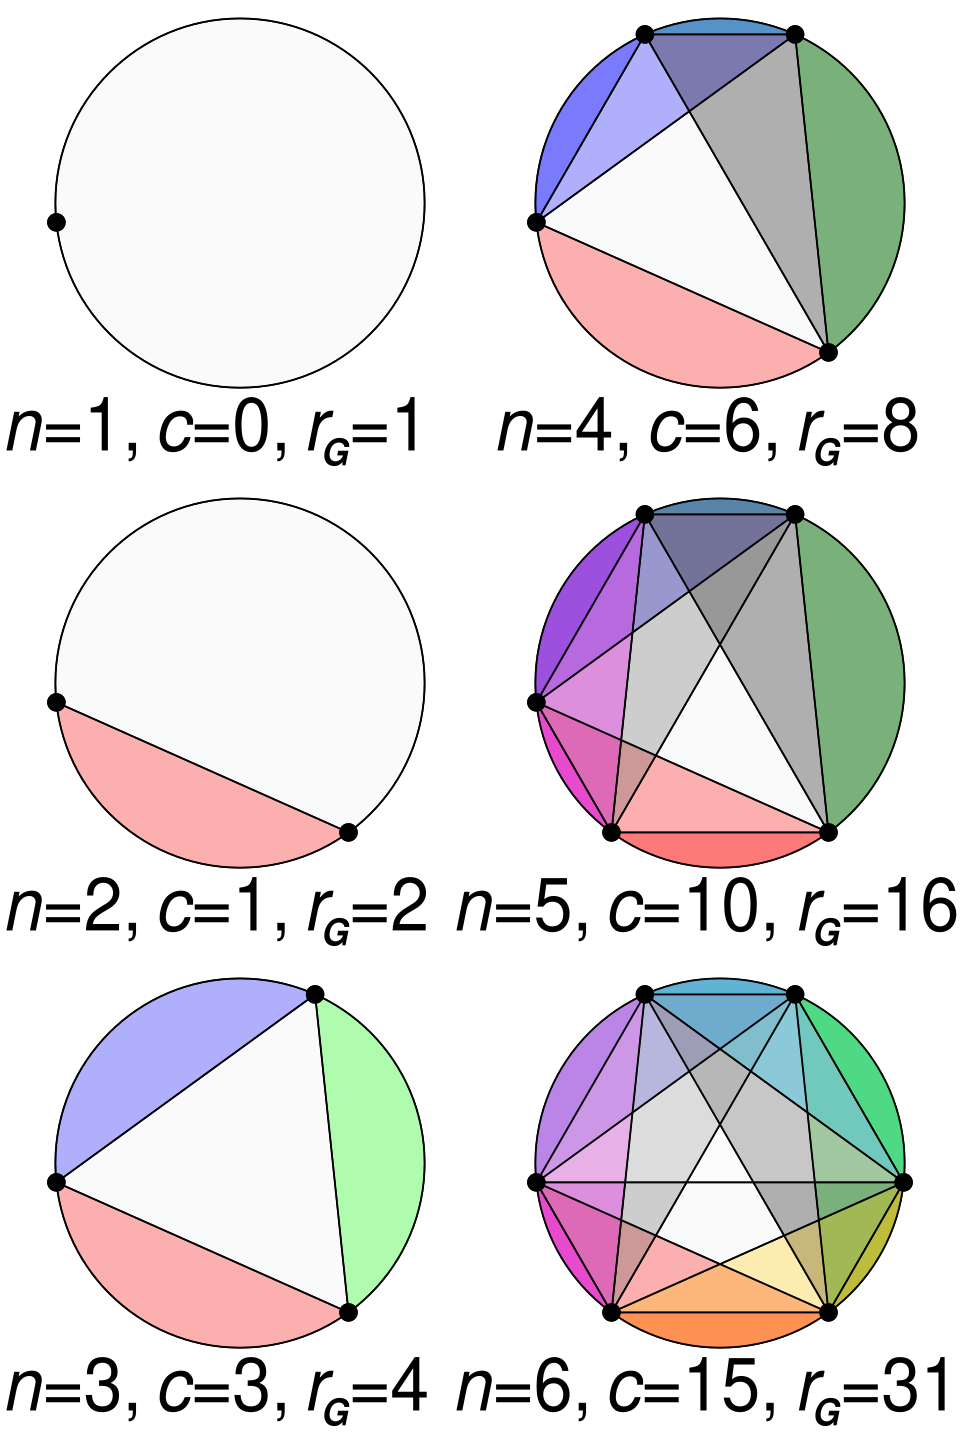
\includegraphics[height=0.50\textheight]{images/Circle_division_by_chords.svg.png} 
\end{figure}
On obtient la séquence $1, 2, 4, 8, 16, 31, 57, 99, 163, 256, \dots$ qui invite à éviter les généralisations hâtives. On la doit à Leo Moser en 1949. En fait, on a :
\begin{equation*}
     r_n = {n \choose 4} + {n \choose 2} + 1 = {\frac {1}{24}}(n^{4}-6n^{3}+23n^{2}-18n+24)
\end{equation*}
\end{frame}

\end{document}